\icode{E-MI-SI-L2-261106-002}
如图，长木板倾斜放置，质量均为\(m\)的直角三角形木块和光滑圆球静止放置在斜面上。木块与木板间	的动摩擦因数为\(\mu\)，最大静摩擦力等于滑动摩擦力，当木板倾角为\(\theta\)时，三角形木块恰好沿斜面下滑，则\paren[]

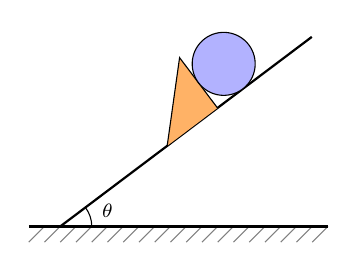
\begin{tikzpicture}[font=\scriptsize]
	\begin{scope}[rotate=37]
		\draw[thick] (0,0)--(4,0);
		\draw[fill=orange!60] (2.5,0)--(2.5,.8)--(1.7,0);
        \draw[fill=blue!30] (2.9,.4) circle(.4);
	\end{scope}
	\foreach \x in {-.4,-.2,...,3.2}
		\draw[gray] (\x,-.2)--++(.2,.2);
	\draw[thick] (-.4,0)--(3.4,0);
	\draw (.4,0) arc(0:37:.4);
	\node at(.6,.2) {\(\theta\)};
\end{tikzpicture}
\begin{choices}
	\item\(\tan\theta = \dfrac{\mu}{2}\)
	\item\(\tan\theta = \mu\)
	\item\(\tan\theta = 2\mu\)
	\item\(\tan\theta = \sqrt{2}\mu\)
\end{choices}
\begin{answer}
	A\qquad 提示：
\end{answer}